\section{Introduction}
\label{sec:intro}

\subsection{Background and Motivation}
\label{intro:sec:background}

The Internet of Things (IoT) has evolved well beyond its early phase, with around 21 billion connected devices in deployment as of 2025, forecast to reach roughly 40 billion by 2030~\cite{iotanalytics2025}. IoT permeates homes, workplaces, farms, Industry 4.0 settings, entertainment venues, and beyond~\cite{IoTfuture, farmbeats, lampropoulos2019internet}. Smart commercial buildings alone account for around 2 billion connected devices today, projected to reach 4.12 billion by 2030, with the building IoT market growing from roughly \$64 billion in 2024 to over \$100 billion by 2030~\cite{memoori2025iot}. As deployments scale, they increasingly span \emph{mesh networks} of heterogeneous devices---smart devices capable of compute and storage alongside simpler devices that only receive commands---creating densely populated edge computing environments across both residential and commercial settings; \Cref{comesh:fig:IoTsetting} illustrates three such commercial settings---a smart building, a smart farm, and a smart factory.

\begin{figure}[th!]
    \centering
    \begin{subfigure}{0.49\linewidth}
        % \vspace{0.2cm}
        \centering
        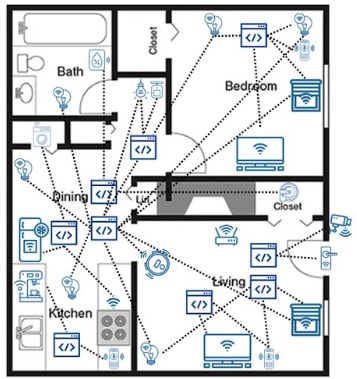
\includegraphics[width=0.75\textwidth,alt={Illustration of a smart home as a residential edge setting, with networked IoT devices distributed across the home.}]{figures/intro/smart-home.png}
        \caption{\small {Smart Home.}}
        \label{comesh:fig:smart-home}
        \medskip
    \end{subfigure}
    \begin{subfigure}{0.49\linewidth}
        \centering
        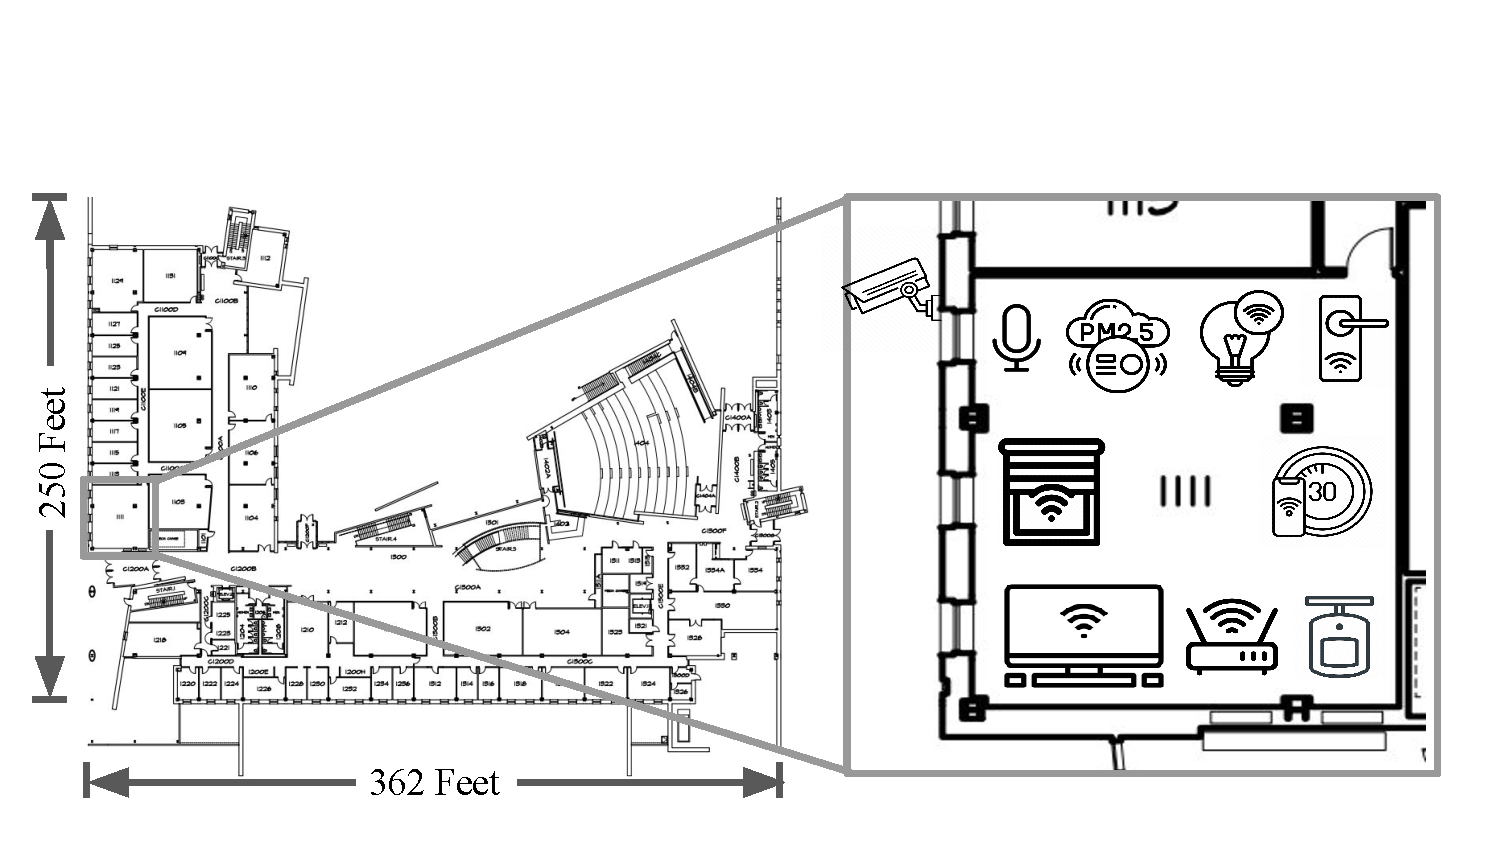
\includegraphics[width=\textwidth,alt={Map/floor plan of a smart office building used as a commercial edge setting, showing the layout across which IoT sensors and actuators are deployed.}]{CoMesh/figures/intro/smart-building.pdf}
        \caption{\small {Smart Building.}}
        \medskip
        \label{comesh:fig:smart-building}
    \end{subfigure}
    \begin{subfigure}{0.49\linewidth}
        \centering
        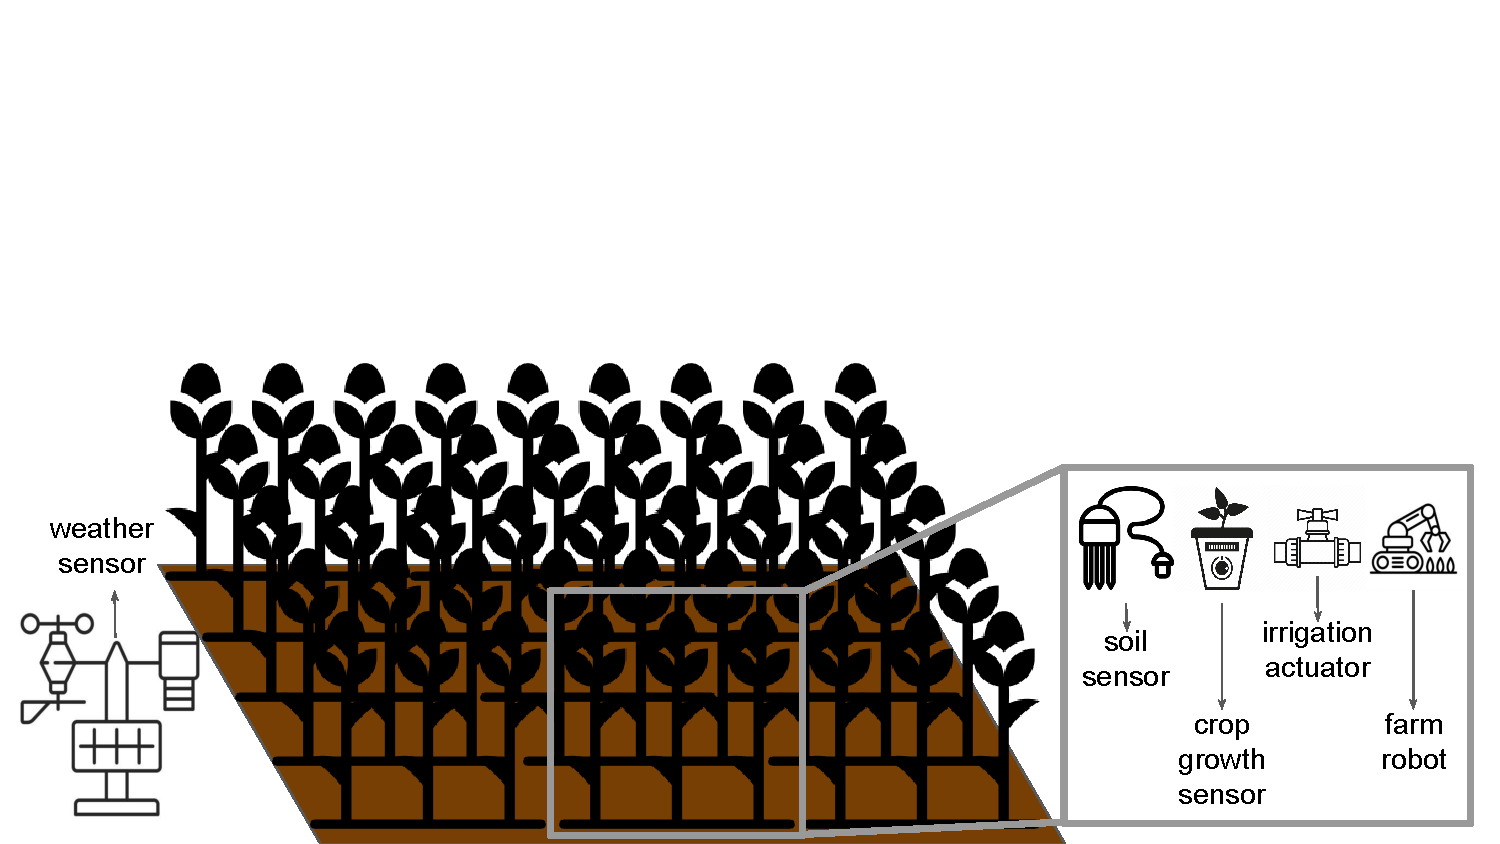
\includegraphics[width=\textwidth,alt={Map of a smart farm used as a commercial edge setting, showing the fields and areas across which IoT sensors and actuators are distributed.}]{CoMesh/figures/intro/smart-farm.pdf}
        \caption{\small {Smart Farm.}}
        \label{comesh:fig:smart-farm}
    \end{subfigure}
    \begin{subfigure}{0.49\linewidth}
        % \vspace{0.2cm}
        \centering
        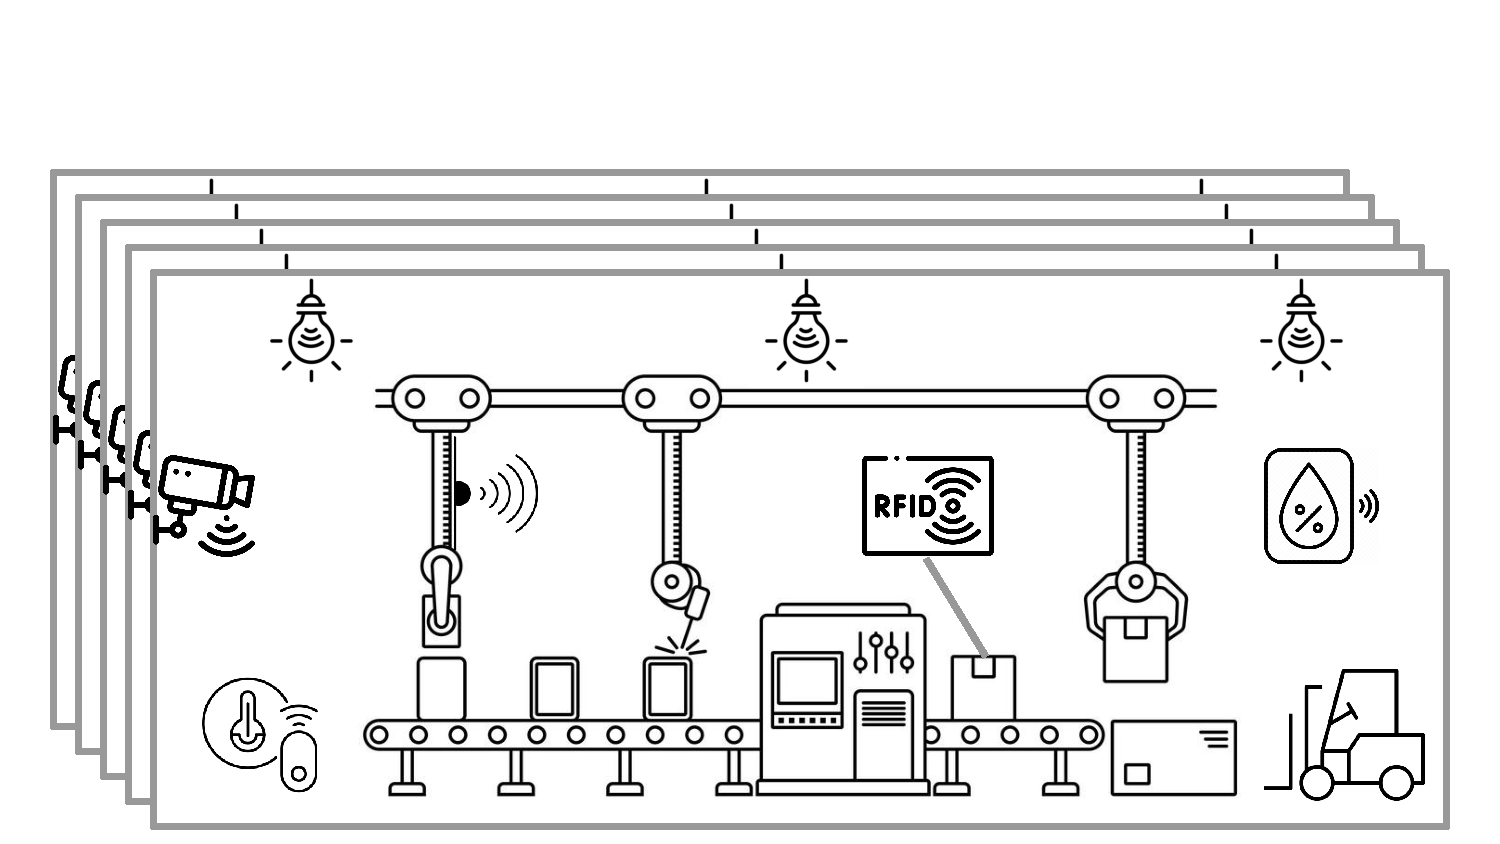
\includegraphics[width=\textwidth,alt={Illustration of a smart factory as a commercial edge setting, with networked industrial IoT devices distributed across the production floor.}]{CoMesh/figures/intro/smart-factory.pdf}
        \caption{\small {Smart Factory.}}
        \label{comesh:fig:smart-factory}
    \end{subfigure}
    \caption{\bf \small Four Edge Settings:
    (a) Smart Home~\cite{iotanalytics2025}, (b) Smart Building~\cite{Memoori}, (c)  Smart Farm~\cite{SMG21}, (d) Smart  Factory~\cite{lampropoulos2019internet}. {\it The Smart Building map from (b) and Smart Farm from (c) drive the experiments in the CoMesh chapter (\ref{chapter:comesh}). }
    }
    \label{comesh:fig:IoTsetting}
    \bigskip
\end{figure}

\begin{table}[th!]
    \centering
    \caption{\bf \small Taxonomy of smart spaces addressed in this thesis and the control challenges each presents.}
    \bigskip
    \label{intro:tab:taxonomy}
    \tagpdfsetup{table/header-rows={1},table/header-columns={1}}
    % \tagpdfsetup{table-tagging=false}
    \begin{tabularx}{\linewidth}{p{0.3\linewidth}p{0.45\linewidth}p{0.15\linewidth}}
        \toprule
        \textbf{Smart Space} & \textbf{Key Control Challenges} & \textbf{This Thesis} \\
        \midrule
        Residential home \par (10s of devices)   & Navigating the control spectrum; \par debugging silent automation failures & \ref{chapter:cic}, \par \ref{chapter:rasc} \\[2pt]
        \midrule
        Commercial building \par (100s--1000s)   & Hub overload; cloud dependency; \par control scalability                   & \ref{chapter:comesh}, \par \ref{chapter:rasc} \\[2pt]
        \midrule
        Smart farm \par (distributed, outdoors)  & Connectivity gaps; \par unattended local operation                         & \ref{chapter:comesh}, \par \ref{chapter:rasc} \\[2pt]
        \midrule
        Smart factory \par (industrial)          & Strict data-locality requirements; \par operational continuity             & \ref{chapter:comesh}, \par \ref{chapter:rasc} \\
        \bottomrule
    \end{tabularx}
\end{table}

We use the term \emph{smart space} to refer to any physical environment instrumented with IoT devices for automated sensing and actuation. Smart spaces span a wide range of scales and deployment contexts---from a residential home with a few dozen consumer devices to a commercial smart building with hundreds or thousands of sensors and actuators, to smart farms and industrial factories with large physical footprints. \Cref{intro:tab:taxonomy} provides a taxonomy of the smart space types addressed in this thesis.

Despite their differences in scale and purpose, all smart spaces share a common computational substrate: the \emph{Sense-Trigger-Actuate} (STA) paradigm, in which devices sense their environment, automation rules evaluate conditions and fire, and commands actuate devices. These workloads---packaged as automations, routines, or scripts---are how occupants and operators program their environments to respond to the world around them.

Modern IoT stacks must be evaluated through two complementary lenses. \textbf{System-facing metrics}---latency, reliability, fault-tolerance, privacy, and cost-efficiency---ensure that automations trigger promptly, survive device or network failures, and protect sensitive telemetry. \textbf{User-facing metrics}---fine-grained control, observability, debuggability, and overall usability---determine whether occupants can understand and shape the behavior of their increasingly complex environments. Together, these metrics define the standard against which any scalable, human-centered IoT platform must be evaluated. This thesis contributes to both dimensions, combining systems design and implementation with empirical human-computer interaction (HCI) research.

Today's dominant IoT architecture routes every sensor reading and actuation request through a vendor cloud backend, which creates three intertwined pain points. First, \textbf{privacy risks} arise because raw telemetry must transit and persist in third-party infrastructure; keeping control logic on-premise eliminates this exposure entirely~\cite{HACloudless, csa2025matter}. In high-security industrial settings---semiconductor fabs and pharmaceutical facilities, for instance---operators routinely prohibit any data from leaving the premises to protect proprietary processes, a constraint cloud-centric platforms cannot satisfy by design. Second, \textbf{reliability degrades} when every automation depends on an Internet path, particularly during network or cloud service outages~\cite{gcloud-down1}. Third, \textbf{cost scales unfavorably}: servicing 500 devices that ping once per second can incur fees approaching \$2{,}500 per month on mainstream IoT cloud tiers~\cite{AzureIoTHub}, while local control removes usage-based bills altogether. Together, these pressures make edge-native, on-premise control an attractive foundation for smart environments that must be private, dependable, and economically sustainable. Crucially, the hardware needed to realize this vision is already in place: smart devices in both residential and commercial settings sit idle for the vast majority of their operational lifetime~\cite{hyperedge}, offering a ready substrate for distributed control logic without requiring any additional infrastructure investment.

Beyond infrastructure placement, the programmability of smart spaces remains a fundamental challenge. IoT automations---routines that chain sensor readings to device actuations\allowbreak ---are central to how occupants live with their environments. Yet the tools available to both users and developers today are impoverished in two ways. First, users navigate a rich spectrum of control options, from physical device interfaces to centralized proxy-based hubs, with limited system support for moving between them fluidly. Platforms today are designed around vendor ecosystems and commercial integration goals, not around the actual, context-dependent ways people rely on their devices. Second, the control primitive underlying virtually all automation platforms---the Remote Procedure Call (RPC)---gives no feedback on whether a physical action has actually taken effect~\cite{birrell1984implementing}. This leaves both users and developers without the observability needed to build reliable, debuggable workflows. Closing these gaps is the central challenge this thesis addresses.

\smallskip\noindent\textbf{Thesis Statement.}
This thesis is the first to drive network and systems design for smart spaces attuned to the needs of the people who inhabit them, advancing this vision across three \emph{independent} planes of the smart-space stack. At the \emph{device action plane}, RASC introduces a control abstraction that brings action-level observability and programmability to IoT automations. At the \emph{smart-space automation plane}, CoMesh provides a decentralized infrastructure that removes hub bottlenecks and cloud dependence. Finally, at the \emph{human interaction plane}, Control in Context contributes an empirical account of how and why real occupants navigate the control spectrum.


\subsection{Thesis Contributions}
\label{intro:sec:contributions}

% Smart-space control-stack figure for the Introduction (intro:fig:stack).
% Device icons live in figures/intro/*.png ; requires fontawesome5 and the
% tikz libraries arrows.meta, shapes.geometric, fit, backgrounds, calc (loaded in macros.tex).
\newcommand{\devm}[1]{\includegraphics[height=0.6cm]{figures/intro/#1}}
\newcommand{\devs}[1]{\includegraphics[height=0.66cm]{figures/intro/#1}}
\tikzset{
 hub/.pic={\fill[black!82,rounded corners=2.5pt](-0.18,-0.12) rectangle (0.18,0.06);\fill[green!60!black](0.11,-0.03) circle (0.022);\draw[black!82,line width=0.6pt](-0.13,0.06)--(-0.16,0.16);\draw[black!82,line width=0.6pt](0.0,0.06)--(0.0,0.17);},
}

\begin{figure}[th!]
  \centering
  \resizebox{\linewidth}{!}{%
  \begin{tikzpicture}[
  alt={Diagram of the smart-space control stack as four stacked layers joined top to bottom by arrows. Top layer, Control in Context (theme: usability), asks how occupants view and use control interfaces: a person points to a spectrum running from physical device control, through a vendor app, to a hub or cloud, i.e. from physical to proxy-based central control. Second layer, CoMesh (theme: scalability and fault tolerance), asks where control logic should run: a mesh of smart-home devices is organized into two overlapping coteries of compute-capable smart devices that share members (one coterie groups a smart speaker, fridge, and vacuum; the other groups a camera, fridge, and vacuum), while simpler sensors and actuators are interspersed, and there is no central hub. Third layer, RASC (theme: observability and programmability), asks how control logic and occupants observe and program actions: a controller sends an action to a device along an observable lifecycle of Request, Acknowledge, Start, and Complete. Bottom layer, Smart Space, shows the IoT devices, mesh network, and people that the upper layers operate over.},
  font=\sffamily, dlarge/.style={font=\Large}, dmed/.style={font=\large},
  ttl/.style={font=\bfseries}, chref/.style={font=\small, text=black!55},
  q/.style={font=\itshape\small, text=black!75, align=left}, lbl/.style={font=\footnotesize, text=black!65},
  tlbl/.style={font=\scriptsize, text=black!70},
  badge/.style={font=\scriptsize, align=right, anchor=north east, fill=white, draw=gray!45, rounded corners=2pt, inner sep=2.5pt},
  flow/.style={-{Stealth[length=2.6mm]}, gray!65, thick},
]
\def\w{16.5}
\fill[orange!8, draw=orange!55, rounded corners=5pt] (0,1.5) rectangle (\w,-1.5);
\fill[blue!8,   draw=blue!50,   rounded corners=5pt] (0,-1.9) rectangle (\w,-6.2);
\fill[teal!9,   draw=teal!55,   rounded corners=5pt] (0,-6.6) rectangle (\w,-10.0);
\fill[gray!12,  draw=gray!60,   rounded corners=5pt] (0,-10.4) rectangle (\w,-14.2);
\draw[flow] (1.9,-1.5) -- (1.9,-1.9);
\draw[flow] (1.9,-6.2) -- (1.9,-6.6);
\draw[flow] (1.9,-10.0) -- (1.9,-10.4);

% ===== L1 Control in Context =====
\node[ttl, anchor=west] at (0.35,0.85) {Control in Context};
\node[chref, anchor=west] at (0.35,0.3) {\ref{chapter:cic}};
\node[q, anchor=west, text width=4.8cm] at (0.35,-0.5) {How do occupants view and use control interfaces?};
\node[badge] at (\w-0.15,1.42) {\textbf{Human interaction plane}\\\itshape usability};
\node[dlarge] (u1) at (6.2,0.2) {\faIcon{user}};
\node (c1) at (8.6,0.35) {\devm{smart-bulb}};
\node[dmed] (c2) at (11.2,0.4) {\faIcon{mobile-alt}};
\node (c3) at (14.0,0.4) {\tikz{\path(0,0) pic[scale=1.25]{hub};}};
\node[tlbl] at (8.6,-0.25) {device};
\node[tlbl] at (11.2,-0.2) {vendor app};
\node[tlbl] at (14.0,-0.25) {hub / cloud};
\draw[flow] (u1) -- (7.5,0.2);
\draw[{Stealth[length=2mm]}-{Stealth[length=2mm]}, black!55] (7.8,-0.8) -- (14.6,-0.8);
\node[tlbl] at (8.6,-1.1) {physical};
\node[tlbl] at (13.4,-1.1) {proxy-based (central)};

% ===== L2 CoMesh : same device mesh + overlapping coteries =====
\node[ttl, anchor=west] at (0.35,-2.7) {CoMesh};
\node[chref, anchor=west] at (0.35,-3.25) {\ref{chapter:comesh}};
\node[q, anchor=west, text width=4.8cm] at (0.35,-4.1) {Where should control\\logic run?};
\node[badge] at (\w-0.15,-1.98) {\textbf{Smart-space automation plane}\\\itshape scalability \& fault tolerance};
\begin{scope}[yshift=-0.5cm]
\node (cspk) at (6.7,-3.6) {\devm{smart-coffee-maker}};
\node (cbu)  at (7.4,-2.5) {\devm{smart-bulb}};
\node (ccf)  at (8.1,-4.3) {\devm{smart-speaker}};
\node (cfr)  at (9.5,-3.5) {\devm{smart-fridge}};
\node (cvac) at (9.9,-4.4) {\devm{smart-vacuum}};
\node (ccam) at (11.3,-3.0){\devm{camera}};
\node (clk)  at (12.7,-3.7){\devm{smart-lock}};
\node (cmo)  at (13.7,-3.0){\devm{motion-sensor}};
\draw[gray!55] (cspk)--(cbu) (cspk)--(ccf) (cbu)--(cfr) (ccf)--(cfr) (ccf)--(cvac) (cfr)--(cvac) (cfr)--(ccam) (cvac)--(ccam) (ccam)--(clk) (ccam)--(cmo) (clk)--(cmo) (cbu)--(ccam);
\node[draw=blue!75, dashed, line width=0.7pt, rounded corners=4pt, fit=(ccf)(cfr)(cvac), inner sep=1.5pt] (cot1) {};
\node[draw=teal!70!blue, dash dot, line width=0.7pt, rounded corners=4pt, fit=(ccam)(cfr)(cvac), inner sep=2.5pt] (cot2) {};
\node[tlbl, text=blue!75] at (8.4,-5.05) {coterie};
\node[tlbl, text=teal!70!blue] at (11.0,-5.05) {coterie};
\node (nh) at (15.2,-3.7) {\tikz{\path(0,0) pic[scale=1.3]{hub};}};
\draw[red!75, very thick] (14.85,-4.0) -- (15.55,-3.4);
\node[lbl, text=red!75] at (15.2,-4.35) {no hub};
\end{scope}

% ===== L3 RASC =====
\begin{scope}[yshift=-0.5cm]
\node[ttl, anchor=west] at (0.35,-6.8) {RASC};
\node[chref, anchor=west] at (0.35,-7.35) {\ref{chapter:rasc}};
\node[q, anchor=west, text width=5.2cm] at (0.35,-8.2) {How do automations and occupants\\observe and program actions?};
\node[badge] at (\w-0.15,-6.18) {\textbf{Device action plane}\\\itshape observability \& programmability};
\begin{scope}[yshift=-0.5cm]
\node[dlarge] (rc) at (6.8,-7.3) {\faIcon{server}};
\node[lbl] at (6.8,-7.95) {control};
\node (rd) at (9.5,-7.3) {\devm{smart-bulb}};
\node[lbl] at (9.5,-7.95) {device};
\draw[flow] (rc) -- (rd);
\draw[teal!60, thick] (10.1,-7.3) -- (15.6,-7.3);
\foreach \x/\l in {10.4/R, 11.6/A, 12.9/S, 15.4/C}{
  \node[circle, fill=teal!60, inner sep=1.7pt] at (\x,-7.3){};
  \node[text=teal!80, font=\footnotesize\bfseries] at (\x,-6.95){\l};}
\node[lbl] at (13.0,-8.0) {Request $\cdot$ Ack $\cdot$ Start $\cdot$ Complete};
\end{scope}
\end{scope}

% ===== L4 Smart Space : same mesh, no coteries =====
\begin{scope}[yshift=-1.7cm]
\node[ttl, anchor=west] at (0.35,-9.8) {Smart Space};
\node[lbl, anchor=west, text width=4.8cm] at (0.35,-11.0) {IoT devices +\\ mesh network +\\ people};
\node[dlarge] (ehum) at (15.1,-10.6) {\faIcon{user}};
\node (espk) at (6.9,-10.6) {\devs{smart-coffee-maker}};
\node (ebu)  at (7.4,-9.5) {\devs{smart-bulb}};
\node (ecf)  at (8.1,-11.3) {\devs{smart-speaker}};
\node (efr)  at (9.5,-10.5) {\devs{smart-fridge}};
\node (evac) at (9.9,-11.4) {\devs{smart-vacuum}};
\node (ecam) at (11.3,-10.0){\devs{camera}};
\node (elk)  at (12.7,-10.7){\devs{smart-lock}};
\node (emo)  at (13.7,-10.0){\devs{motion-sensor}};
\draw[gray!50] (espk)--(ebu) (espk)--(ecf) (ebu)--(efr) (ecf)--(efr) (ecf)--(evac) (efr)--(evac) (efr)--(ecam) (evac)--(ecam) (ecam)--(elk) (ecam)--(emo) (elk)--(emo) (ebu)--(ecam);
\end{scope}
\end{tikzpicture}}
  \caption{\bf \small Three user-aware planes of smart-space control, designed around the needs of the people who inhabit the space.
    {\it The \emph{device action plane} (RASC) exposes each action's Request-Ack-Start-Complete lifecycle; the \emph{smart-space automation plane} (CoMesh) decentralizes where control logic runs; and the \emph{human interaction plane} (Control in Context) characterizes how occupants view and use control interfaces. All three operate over a shared smart space of devices, mesh network, and people.}}
  \bigskip
  \label{intro:fig:stack}
\end{figure}


\begin{table}[th!]
    \centering
    \caption{\bf \small Contributions of this thesis, their objectives, and evaluation methodology.}
    \bigskip
    \label{intro:tab:contributions}
    \tagpdfsetup{table/header-rows={1},table/header-columns={1}}
    % \tagpdfsetup{table-tagging=false}
    \renewcommand{\arraystretch}{1.3}
    \renewcommand{\tabularxcolumn}[1]{m{#1}}
    \begin{tabularx}{\linewidth}{>{\raggedright\arraybackslash}m{2.3cm}|>{\raggedright\arraybackslash}m{2.3cm}|X|>{\raggedright\arraybackslash}m{2.6cm}|>{\raggedright\arraybackslash}m{1.9cm}}
        \hline
        \textbf{Work} & \textbf{Plane} & \textbf{Objective} & \textbf{Evaluation} & \textbf{Venue} \\
        \hline\hline
        RASC~\cite{rasc}
        & Device action
        & {\small Observability \& programmability abstraction for IoT device actions}
        & System\par measurements
        & {\footnotesize USENIX\par NSDI 2026} \\
        \hline
        CoMesh~\cite{comesh}
        & Smart-space automation
        & {\small Scalable \& fault-tolerant abstraction for commercial edge IoT mesh automations}
        & System\par measurements
        & {\footnotesize IEEE\par TNSM 2026} \\
        \hline
        Control in Context~\cite{controlincontext}
        & Human interaction
        & {\small Smart home control-interface navigation framework}
        & HCI analysis
        & {\footnotesize ACM\par CHI 2026} \\
        \hline
    \end{tabularx}
\end{table}

This thesis makes three concrete contributions to the control of smart spaces---one at each plane of the smart-space stack, unified by a single user-aware vision (\Cref{intro:fig:stack}). It combines systems design and implementation with empirical user research. \Cref{intro:tab:contributions} summarizes the three contributions and their evaluation methodology.

\begin{itemize}
    \item \textbf{The device action plane: observable, programmable control (\ref{chapter:rasc}).}
    \emph{How do automations and occupants observe and program actions?}
    The RPC primitive underlying all IoT platforms is fire-and-forget, leaving developers and occupants without feedback on whether actions have actually taken effect. RASC~\cite{rasc} is a new control abstraction that exposes the full action lifecycle, so that automations---and the people who write them---can observe whether an action started, completed, or failed, and program causal dependencies among actions, all without requiring any device modifications.

    \item \textbf{The smart-space automation plane: scalable, fault-tolerant control (\ref{chapter:comesh}).}
    \emph{Where should control logic run?}
    Today's platforms concentrate control logic in a central hub or cloud, creating bottlenecks, single points of failure, and cloud dependency. CoMesh~\cite{comesh} is the first fully decentralized, hub-less control plane for large commercial edge IoT meshes: it spreads control across the devices themselves, so the system \emph{scales} to thousands of devices and \emph{tolerates} device failures, churn, and mobility without any central point of failure.

    \item \textbf{The human interaction plane: usable control interfaces (\ref{chapter:cic}).}
    \emph{How do occupants view and use control interfaces?}
    Smart home users interact through a spectrum of command interfaces---from pressing a physical button on a device, to a per-brand mobile app, to a centralized hub application such as Google Home or Alexa that routes all commands through a cloud backend.
    These represent different interface architectures, each with different latency, reliability, and failure-mode characteristics.
    System designers have long assumed centralized hub interfaces are users' primary mode, yet real behavior is far more nuanced.
    Control in Context~\cite{controlincontext} is the first empirical characterization of how and why users move across this interface spectrum in practice, grounding future interface and system design in observed behavior rather than assumptions.
\end{itemize}

These are independent contributions unified by a single vision---user-aware design---rather than a pipeline: no insight ``flows'' from one to the next, and none subsumes another. Together they make three planes of the smart-space stack---the \emph{device action plane} (how actions are observed and programmed), the \emph{smart-space automation plane} (where control logic runs), and the \emph{human interaction plane} (how occupants view and use control interfaces)---resilient, observable, and built around the people who inhabit the space. \Cref{intro:fig:stack} situates each contribution accordingly.


\subsubsection{RASC: Enhancing Observability and Programmability in Smart Spaces}
\label{intro:sec:rasc}

IoT platforms today rely on RPC, a fire-and-forget primitive that provides no feedback on whether a physical action has started, completed, or failed. This leaves both users and developers without the observability needed to build reliable routines, reason about device state, or diagnose failures. We introduce RASC~\cite{rasc} (Request-Ack-Start-Complete), a new abstraction for IoT device control that exposes the full lifecycle of every action, and Rascal, its implementation atop existing RPC-based IoT platforms.

RASC's contributions are:
\begin{itemize}
    \item The RASC abstraction, which extends RPC with four lifecycle states---Request, Acknowledgment, Start, and Complete---enabling both users and higher-level automation systems to reason about action progress in real time.
    \item An adaptive polling strategy that detects when actions start, complete, or fail with minimal overhead, without requiring any device-side modifications.
    \item Scheduling policies over a directed acyclic graph (DAG) of actions that express causal dependencies, enabling routines that react dynamically to action outcomes rather than relying on fixed time windows.
    \item Integration with Home Assistant via Rascal, a widely used open-source smart home platform, and trace-driven evaluation showing that Rascal detects action completion within 2--16 seconds over 90\% of cases and that its scheduling policies outperform state-of-the-art baselines by 10--55\%.
\end{itemize}


\subsubsection{CoMesh: A Decentralized Control Plane for Commercial Edge IoT Meshes}
\label{intro:sec:comesh}

Today's smart spaces route all STA coordination through a central hub or cloud---a single point of failure that drives outages, exposes private telemetry, and incurs prohibitive cloud costs, and that does not scale to the hundreds-to-thousands of devices in commercial edge deployments such as smart buildings, farms, and factories. We present CoMesh~\cite{comesh}, the first fully decentralized, hub-less control plane for STA operations over large commercial edge IoT meshes. CoMesh organizes smart devices into overlapping subgroups called \emph{coteries} that collectively monitor devices and manage routines using zero-message exchange protocols, quorum-based agreement, epoch-based migration, and locality-sensitive hashing (LSH). The result is a self-healing architecture that adapts to device failures, churn, and mobility without human intervention.

CoMesh's contributions are:
\begin{itemize}
    \item Design and implementation of CoMesh using a novel combination of distributed systems techniques: load-balanced STA operations over space and time; zero-message member selection; quorum-based agreement; and LSH-based locality to minimize inter-device communication.
    \item Formal proofs of CoMesh's safety, liveness, and progress properties.
    \item Experimental evaluation on Raspberry Pi deployments and large-scale simulations using real building maps and automation workloads, demonstrating scalability, fault-tolerance, and low latency.
\end{itemize}


\subsubsection{Control in Context: How Smart Home Users Navigate Proxy-Based Control Schemes}
\label{intro:sec:cic}

Smart home platforms are designed around vendor ecosystems and commercial integration goals, not the actual, context-dependent ways people live with and rely on their devices. Prior work examined individual control schemes in isolation or proposed system architectures without grounding them in observed user behavior. We present Control in Context~\cite{controlincontext}, a mixed-methods study characterizing how and why smart home users navigate the spectrum from physical device interaction to proxy-based centralized control across everyday tasks, device failures, and evolving home setups.

Control in Context's contributions are:
\begin{itemize}
    \item A survey of $N=60$ smart home device owners and semi-structured follow-up interviews with $N=8$ participants, revealing that control is a fluid, reflective process shaped by tradeoffs between convenience, reliability, and cognitive load.
    \item Evidence that users move freely along the control spectrum guided by situational factors such as task type, perceived reliability, and device location---not by abstract ecosystem boundaries.
    \item Characterization of how troubleshooting workflows interact with control scheme preferences, showing that failures lead users to reassess strategies and sometimes abandon devices or platforms entirely.
    \item Design implications for future smart home systems that support movement across the control spectrum and treat the user---not the device ecosystem---as the center of design.
\end{itemize}


\subsection{Broader Impact}
\label{intro:sec:impact}

This thesis advances a local-first, human-centered vision for IoT, with benefits for commercial ecosystems, everyday occupants, and the research community:

\begin{itemize}
    \item \textbf{Progress-aware automation (RASC):}
    \begin{itemize}
        \item Multi-vendor automation tooling without brittle polling or closed software development kits.
        \item Fewer silent failures: occupants can inspect, pause, or roll back automations like debugged programs.
        \item A common API for reasoning about---and formally verifying---workflow correctness.
    \end{itemize}

    \item \textbf{Decentralized edge control (CoMesh):}
    \begin{itemize}
        \item Runs on the idle devices already present~\cite{hyperedge}---no recurring cloud fees, less wide-area network traffic, and no single-hub failure point.
        \item Keeps sensitive telemetry on-premises, easing regulatory exposure.
        \item Keeps critical automations (locks, alarms) working through network and cloud outages.
        \item Seeds sustainable, low-carbon IoT research---constrained, mostly-idle devices can shoulder control once reserved for data centers.
    \end{itemize}

    \item \textbf{Human-centered control insights (Control in Context):}
    \begin{itemize}
        \item Ground-truth evidence on where occupants struggle cuts device returns and support volume.
        \item Motivates transparency-driven designs that make dense smart spaces accessible and trustworthy for less-technical users.
        \item Clearer mental models and faster diagnostics for occupants in dense smart spaces.
    \end{itemize}
\end{itemize}

Collectively, this thesis turns once vendor-locked properties---privacy, latency, and programmability---into parameters that occupants and developers can tune to fit their priorities---choosing how intelligent their space is and where that intelligence lives.


\subsection{Thesis Organization}
\label{intro:sec:organization}

The remainder of this dissertation is organized as follows. \ref{chapter:rasc} presents Rascal, our implementation of the RASC abstraction, including case studies, dynamic scheduling algorithms, and a trace-driven evaluation. \ref{chapter:comesh} presents CoMesh, our decentralized control plane for commercial edge IoT meshes, including formal analysis and evaluation on Raspberry Pi deployments and large-scale simulations. \ref{chapter:cic} presents Control in Context, our mixed-methods user study characterizing how and why smart home users navigate the spectrum from physical to proxy-based control. The dissertation concludes with a summary of contributions and a discussion of future directions.
